\documentclass{SINet}
\usepackage{ifthen}
\usepackage[printonlyused,nohyperlinks]{acronym}
\usepackage{lipsum}
\usepackage[utf8]{inputenc}
\usepackage{siunitx}
\usepackage[square,numbers]{natbib}
\usepackage{booktabs}
% added after johan review
\usepackage{textcomp}
\usepackage{eurosym} % use \EUR for euro symbol!
\usepackage{tikz}
    \usetikzlibrary{calc}

\usepackage{tikzpagenodes}

\newcommand{\onlypnum}{%
    \thispagestyle{empty}%
    \begin{tikzpicture}[remember picture, overlay]
        \node at (current page footer area.south east) [
            anchor=base,
        ] {
            \thepage
        };
    \end{tikzpicture}%
    \ignorespaces
}
\hyphenation{FashionBrain science participant}
\pretolerance=5000
\tolerance=9000
\emergencystretch=0pt
\righthyphenmin=4
\lefthyphenmin=4
% end johan review

\newcommand{\ra}[1]{\renewcommand{\arraystretch}{#1}}
\usepackage[section]{placeins}
\usepackage[figure,table]{totalcount}
\usepackage [english]{babel}
\usepackage{xurl}
\usepackage [autostyle, english = american]{csquotes}
\MakeOuterQuote{"}
\usepackage{totpages}
\usepackage{totcount}
\usepackage[nottoc]{tocbibind}
\newcommand{\say}[1]{\begin{center}\par\begin{minipage}{0.8\columnwidth}\blockquote{#1}{}\end{minipage}\end{center}}
\newtotcounter{acronum}
\def\oldac{} \let\oldac=\ac
\def\ac{\stepcounter{acronum}\oldac}
\def\oldused{} \let\oldused=\acronymused
\def\acronymused{\stepcounter{acronum}\oldused}



\newcommand{\mkh}[1]{\textcolor{red}{(*** MK: #1 ***)}}
\newcommand{\iar}[1]{\textcolor{blue}{(*** IAR: #1 ***)}}
\newcommand{\onequote}[1]{`#1'}
\newcommand{\quotes}[1]{``#1''}


% EDIT THIS -------------------------------------------
\newcommand{\DelTitle}{Requirement Analysis Document}
\newcommand{\ShortTitle}{\DelTitle} %change it if needed for a shorter footer
\newcommand{\DelNumber}{D2.2}
\newcommand{\DelVersion}{4.0}
% -----------------------------------------------------

\addto\captionsenglish{%
  \renewcommand{\contentsname}%
    {Table of Contents}%
}

% EDIT THIS -------------------------------------------
% If you want to manually add acronyms to a list without
% using the \ac command in the text, simply add them here:
\acronymused{AR}
\acronymused{CF}
\acronymused{CSV}
\acronymused{ID}
\acronymused{FB}
\acronymused{JSON} 
\acronymused{NLP}
\acronymused{OEM}
\acronymused{RD}
\acronymused{SKU}
\acronymused{SM}
\acronymused{TF-IDF}
\acronymused{VR}
\acronymused{YT}
\acronymused{WP}

%...
% -----------------------------------------------------


\begin{document}
\pagenumbering{roman}
\thispagestyle{plain}
% EDIT THIS -------------------------------------------
% Enter the deliverable information  in this document (title.tex)	% EDIT 

%%%%%%%%%%%%%%%%%%%%%%%%%%%%%%%%%%%%%%%%%%%%%%%%%%%%%%%%%%%%%%%%%%%%%%%%%%%%%%%%%%
% First Page
%%%%%%%%%%%%%%%%%%%%%%%%%%%%%%%%%%%%%%%%%%%%%%%%%%%%%%%%%%%%%%%%%%%%%%%%%%%%%%%%%%

\graphicspath{{images/}}
\graphicspath{{images/logos/}{images/figs/}}


\newcommand{\footertext}{\raisebox{3mm}{\DelNumber{} -- \ShortTitle}}
\setlength{\footheight}{36pt}
\newcommand{\footerlogo}{\raisebox{3mm}{\leavevmode
\includegraphics[width=2cm]{logo_white}}}
\clearscrheadfoot
\pagestyle{empty}
\thispagestyle{plain}

% \begin{tikzpicture}[overlay,remember picture]
%   \draw [line width=1pt]
%   ($ (current page.north west) + (1cm,-1cm) $)
%   rectangle
%   ($ (current page.south east) + (-1cm,1cm) $);
% \end{tikzpicture}

\definecolor{SINetblue}{HTML}{07505B} 
\newcolumntype{C}{ >{\centering\arraybackslash} m{4cm} }

\begin{center}
Horizon 2020
\vspace{2cm}

  \begin{center}



  
\includegraphics[width=0.7\textwidth]{logo_white.pdf}
  \vspace{2mm}

  \end{center}
  \vspace{0.5cm}
  {\Large Understanding Europe's Fashion Data Universe\\}
  \vspace{2cm}
  
  \begin{spacing}{2.5}
    \textbf{\Huge \DelTitle}\\\vspace{10mm}
    \textbf{\Large Deliverable number: \DelNumber} \\\vspace{10mm} 
    {\large Version \DelVersion}
  \end{spacing}
  
  \vspace*{\fill}

  %just to avoid warning :)
  \newcommand\undefcolumntype[1]{\expandafter\let\csname NC@find@#1\endcsname\relax}
  \newcommand\forcenewcolumntype[1]{\undefcolumntype{#1}\newcolumntype{#1}}
  \forcenewcolumntype{C}{ >{\arraybackslash} m{3cm} }


  \begin{tabular}{C@{\hspace*{0cm}}l}
    
\includegraphics[scale=0.2]{images/logos/EU_Flag_320_213} &
    \begin{tabular}{l}
    {Funded by the European Union’s Horizon 2020 research and }\\
    {innovation programme under Grant Agreement No. 732328}\\
    \end{tabular}
  \end{tabular}
\end{center}

\clearpage

%%%%%%%%%%%%%%%%%%%%%%%%%%%%%%%%%%%%%%%%%%%%%%%%%%%%%%%%%%%%%%%%%%%%%%%%%%%%%%%%%%
% Second Page 
%%%%%%%%%%%%%%%%%%%%%%%%%%%%%%%%%%%%%%%%%%%%%%%%%%%%%%%%%%%%%%%%%%%%%%%%%%%%%%%%%%

\setlength{\headheight}{1cm}
\setlength{\footskip}{18mm}
\addtolength{\textheight}{-\footskip} \pagestyle{empty}
% add johan
\onlypnum
% end johan

\begin{flushleft}
  \begin{tabular}{ll}
    \textbf{Project Acronym:}       &   FashionBrain \\
    \textbf{Project Full Title:}    &   Understanding Europe's Fashion Data Universe  \\
    \textbf{Call:}                  &   H2020-ICT-2016-1 \\ 
    \textbf{Topic:}                 &   ICT-14-2016-2017, Big Data PPP: Cross-sectorial and \\
& cross-lingual data integration and experimentation  \\
%    \textbf{Type of Action:}        &   RIA \\
%    \textbf{Grant Number:}          &   699924 \\
    \textbf{Project URL:}           &  \url{https://fashionbrain-project.eu} 
  \end{tabular}



% define "struts", as suggested by Claudio Beccari in
%    a piece in TeX and TUG News, Vol. 2, 1993.
\newcommand\Tstrut{\rule{0pt}{2.6ex}}         % = `top' strut
\newcommand\Bstrut{\rule[-0.9ex]{0pt}{0pt}}   % = `bottom' strut



% EDIT THIS -------------------------------------------
  \begin{tabular}{|l|p{100mm}|}\hline
   % \Tstrut\Bstrut Editor& XXX, XXX-Institution\\\hline
    \Tstrut\Bstrut Deliverable type& Report (R) \\\hline
    \Tstrut\Bstrut Dissemination level& Public (PU)\\\hline
    \Tstrut\Bstrut Contractual Delivery Date& 30 June 2018\\\hline
    \Tstrut\Bstrut Resubmission Delivery Date& 27 February 2019\\\hline
    % \Tstrut\Bstrut Suggested Readers:&Project partners, future community-lab.net users\\\hline
    \Tstrut\Bstrut Number of pages&\ref{TotPages}, the last one
being no. \pageref{TotPages}\\\hline
    %\Tstrut\Bstrut Keywords:& XXX \\\hline
    \Tstrut Authors&
 \begin{tabular}{l}
     Ines Arous, Mourad Khayati - UNIFR \Bstrut
     \\
    \end{tabular}\\\hline
    \Tstrut\Bstrut Peer review &
    \begin{tabular}[t]{l}
		Alessandro Checco, Jennifer Dick - USFD\\ Jennie Zhang - MDBS\\
	\end{tabular}\\\hline
  \end{tabular}
% -----------------------------------------------------
  
  
\end{flushleft}

% EDIT THIS -------------------------------------------
\section*{Change Log}
\begin{tabular}{|c|c|c|c|c|}\hline
    \textbf{Version} & \textbf{Date} & \textbf{Status} & \textbf{Partner} &  \textbf{Remarks}\\\hline
      0.1 & 01/08/2017& Draft& UNIFR &  \\\hline
      1.0 & 08/09/2017& Final & UNIFR,  USFD, Zalando & Rejected 15/03/2018  \\\hline
      2.0 & 20/04/2018&  Resubmitted Final & UNIFR, USFD & Rejected 26/04/2018 \\\hline
      3.0 & 21/05/2018& Resubmitted Final & UNIFR, USFD & Rejected 15/10/2018\\\hline
      3.1 & 15/02/2018& Revised Draft & UNIFR, USFD, Zalando& \\\hline
      4.0 & 27/02/2019& Resubmitted Final & UNIFR, USFD, Zalando&  \\\hline
  \end{tabular}
\section*{Deliverable Description}
This deliverable will consist of an extended requirement analysis document detailing expert sourcing. It will collect requirements based on the data sources identified in WP1 (T1.1) and it will feed into WP3.
% -----------------------------------------------------
\clearpage


% -----------------------------------------------------

\refoot[\pagemark]{\pagemark}
\rofoot[\pagemark]{\pagemark}

\section*{Abstract}
%add johan DO NOT REMOVE
\thispagestyle{plain}
%end johan


In the context of the FashionBrain project, several datasets have been provided by our partners which
will be used in order to perform different tasks such as extract key features from text and/or images, capture customers’ preferences or predict new fashion trends as they emerge on social media and the blogosphere.  In this deliverable,
we describe these datasets (size, format, properties, etc.) and we explain how  to identify and expand the sources of data relevant to the domain of fashion by means of crowdsourcing. We conducted a survey in order to assess the importance of social media in the online shopping experience. As a result, we are able to extract the most important social media platforms as well as the most important features in online shopping. 


\setcounter{tocdepth}{2}

\tableofcontents
\iftotalfigures\listoffigures\fi
\begingroup
\let\clearpage\relax
\iftotaltables\listoftables\fi
\endgroup

\ifnum\totvalue{acronum}>0%
% EDIT ME HERE: https://www.overleaf.com/8548773748ymqchwgtzxts
%
%
%% COMMANDS
%%
%% \acresetall	flushes the ’memory’ of the macro \ac (ie all "used" marks flushed)
%%
%% \ac{label}	singular (first time Full Name + (ACRO) and mark as used)
%% \acp{label}	plural (as \ac but makes short and/or long forms into plurals)
%%
%% \acs{lable}	short (ACRO)
%% \acf{lable}	“full acronym” (Full Name + (ACRO))
%% \acl{lable}	long (_without_ ACRO)
%%
%% \acsp{label}	short plural (ACROs)
%% \acfp{label}	“full acronym” plural (Full Names + (ACROs))
%% \aclp{label}	long plural (_without_ ACRO)
%%
%% \acrodef{label}[acronym]{written out form}	definition
%%		for example \acrodef{etacar}[$\eta$ Car]{Eta Carinae},
%%		with the restriction that the label should be simple ASCII


%% PACKAGE & OPTIONS
%% acronym package must be loaded (in the preamble):
%%    \usepackage[option1,option2,etc.]{acronym}
%% OPTIONS:
%%    footnote		The option footnote makes the full name appear as a
%%			footnote.
%%    nohyperlinks	If hyperref is loaded, all acronyms will link to their
%%			glossary entry. With the option nohyperlinks these
%%			linkscan be suppressed.
%%    printonlyused	Only list used acronyms
%%    withpage		In printonlyused-mode show the page number where
%%			each acronym was first used.
%%    smaller		Make the acronym appear smaller.
%%    dua			The option dua stands for “don’t use acronyms”. It
%%			leads to a redefinition of \ac and \acp, making the
%%			full name appear all the time and suppressing all
%%			acronyms but the explicity requested by \acf or \acfp.
%%    nolist		The option nolist stands for “don’t write the list of
%%			acronyms”.


%% INCLUSION
%%
\clearpage
\phantomsection
\addcontentsline{toc}{chapter}{List of Acronyms and Abbreviations}
\chapter*{List of Acronyms and Abbreviations}
\label{sec:acronyms}

\begin{acronym}[OMNeTXX] %width of the longest acronym should be matched here
% PLEASE INSERT THEM IN ALPHABETIC ORDER
% NOTE \acroextra content will be shown only on the list, not on the expansion in the text.
        \acro{AR}{Augmented Reality}
        \acro{CF}{Crowdflower (\url{www.crowdflower.com})\acroextra{, micro-task crowdsourcing platform}}
    \acro{CSV}{Comma Separated Values}
    \acro{ID}{Identifier}
    \acro{FB}{Facebook (\url{www.facebook.com})}
     \acro{JSON}{JavaScript Object Notation}    
    \acro{NLP}{Natural Language Processing}
    \acro{OEM}{Original Equipment Manufacturer}
    \acro{RD}[R\&D]{Research and Development}
    \acro{SKU}{Stock Keeping Unit}
    \acro{SM}{Social Media}
    \acro{TF-IDF}{Term Frequency-Inverse Document Frequency}
    \acro{VR}{Virtual Reality}
    \acro{WP}{Work Package}
    \acro{YT}{YouTube (\url{www.youtube.com})}

 

  %\acro{h2o}[$\boldsymbol{\mathrm{H_2O}}$]{water}
  %\acro{HTTP}{Hypertext Transfer Protocol}


\end{acronym}
\clearpage
\fi

\clearscrheadfoot 
\lofoot[\footerlogo \hspace{10pt} \footertext]{\footerlogo \hspace{10pt} \footertext}
\lefoot[\footerlogo \hspace{10pt} \footertext]{\footerlogo \hspace{10pt} \footertext}
\refoot[\pagemark]{\pagemark}
\rofoot[\pagemark]{\pagemark}
\rohead{\rightmark}
\rehead{\rightmark}
\lohead{\leftmark}
\lehead{\leftmark}

\pagenumbering{arabic}
\setcounter{page}{1}
\pagestyle{scrheadings}

% EDIT THIS add the files you need here----------------
\chapter{Introduction}
\label{chap:intro}


%%%%%%%%%%%%%%%%%%%%%%%%%%%%%%%%%%%%%%%%%%%%%%%%%%%%%%%%%%%%%%%%%%%%%%%%%%%%%%%%%%%%%%%%%%%%%
%%%%%%%%%%%%%%%%%%%%%%%%%%%%%%%%%%%%%%%%%%%%%%%%%%%%%%%%%%%%%%%%%%%%%%%%%%%%%%%%%%%%%%%%%%%%%
\section{Motivation of the Deliverable}
\label{sec:motiv}

The fashion domain involves multiple industry players e.g., fashion designers, production chains, retailers, marketing companies, value-added services, \ac{SM} outlets etc. Each player produces important pieces of information that can be used to provide a better end-user experience, improve individual processes and drive more profit. Fashion data has recently gained a lot of attention in various fashion applications e.g., clothing recommendation, clothing recognition, fashion trend prediction, etc. Yet, the relationship between datasets emanating from retailers and social media is rarely explored. One major impediment is the distribution of the data sources containing relevant products information. Once we uncover these datasources, we are still faced with the challenge of integrating them into a federated data repository. For instance, two online retailers might deal with common brands yielding redundant items in their datasets, thus, the need of eliminating redundant data. In the context of the FashionBrain project, the datasets provided by our partners will be used in order to i) automatically process text and image data and extract key features such as fashion items, ii) capture customers’ preferences, iii) build a fashion-based recommendation engine and iv) predict new fashion trends as they emerge on \ac{SM} and the blogosphere. 


%%%%%%%%%%%%%%%%%%%%%%%%%%%%%%%%%%%%%%%%%%%%%%%%%%%%%%%%%%%%%%%%%%%%%%%%%%%%%%%%%%%%%%%%%%%%%
%%%%%%%%%%%%%%%%%%%%%%%%%%%%%%%%%%%%%%%%%%%%%%%%%%%%%%%%%%%%%%%%%%%%%%%%%%%%%%%%%%%%%%%%%%%%%
\chapter{Data Description}
\label{chap:ddesc}

This section depicts the datasets provided by the project’s industrial partners. We give an overview on a retailer and on fashion-tech startup potential datasets. We will also describe the datasets content and focus on their future use in the context of FashionBrain. This section will be briefly extended by introducing the data integration technique that will be deployed. Table~\ref{tab:data-zalando} summarizes the main properties of the datasets provided by Zalando.
\smallskip


\begin{table}[htb]\centering
\def\arraystretch{1.2}
\begin{tabular}{|l|c|c|l|c|}
\hline
 \textbf{File name} & \textbf{Format}  &  \textbf{Size} & \textbf{Brief description} & \textbf{Date} \\
 \hline\hline
 region1\_items & csv  &22.2 MB  &Items classification in Zalando &  31.03.2017  \\
 region2\_items &  &  &anonymized tree with the & \\
 &  &  & amount and \# of items sold  &  \\
 \hline
 region1\_orders & csv  &42 KB  &Items’ orders with the gross  &  31.03.2017  \\
 region2\_orders &  &  &amount  & \\
 \hline
zalando-images- & csv  &1.01 GB  &A detailed identification of  &  24.04.2017  \\
attributes-FB- &  &  &products from different brands& \\
release&  &  & and their specialized features  &  \\
 \hline
zalando-reviews- & csv  &355.2 MB  &Users’ comments on different  &  24.04.2017  \\
FB-release&  &  & products& \\
 \hline
OEM\_ & csv  &5.2 MB  &Mapping of item attributes &  31.03.2017  \\
translations&  &  & rendered in different  & \\
&  &  &  languages on the web site & \\
 \hline
\end{tabular}
\caption{Datasets provided by Zalando.}
\label{tab:data-zalando}
\end{table}
\smallskip

Table~\ref{tab:data-fashwell} summarizes the main properties of the datasets provided by Fashwell.

\begin{table}[htb]\centering
\def\arraystretch{1.2}
\begin{tabular}{|l|c|c|l|c|}
\hline
 \textbf{File name} & \textbf{Format}  &  \textbf{Size} & \textbf{Brief description} & \textbf{Date} \\
 \hline\hline
dump-example- & json &3.6 MB  &A detailed identification of&  30.03.2017  \\
macys &  &  &  products   from “Macys” with & \\
 &  &  &  their specialized features & \\
\hline 
dump-example- & json & 4.3 MB  &A detailed identification of  &  30.03.2017  \\
gap &  &  & products from “GAP” with & \\
 &  &  & their specialized features & \\
\hline 
products-example & json &512 KB &an example of the json  &  30.03.2017  \\
 &  &  & description of a given product  & \\
\hline 
fashion\_tree\_dump& csv &21 KB  &Fashwell Fashion tree  &  04.05.2017  \\
\hline 
products-schema & json &3 KB  &A schema explaining  &  30.03.2017  \\
 &  &  &  the content of the json files  & \\
\hline 
\end{tabular}
\caption{Datasets provided by Fashwell.}
\label{tab:data-fashwell}
\end{table}

\section{Fashion Retailer Data}

This section provides a detailed description of the datasets provided by Zalando and that will be used in order to offer exclusive data services to their customers as they will be able to  anticipate customer needs, and predict short and long term trends or frauds. The datasets are in the form of csv files containing each a table of attributes.  This section will be divided into two parts. In the first part, the attributes of each file will be presented by providing their type and description. Next, we will analyse how these datasets can be used in terms of research. In the second part, we will summarize the relationship between the files in a relational schema.

\subsection{Datasets Analysis}

\paragraph*{OEM\_Translation.csv}: In order to keep a tight relation with its clients, Zalando offers the possibility for users to see product attributes in their own language depending on the localization of the website. The OEM\_Translation file includes items’ attributes rendered in different languages on the website. This file is used to map multilingual description to one fashion vocabulary.

\begin{itemize}
    \item Attribute\_type (String): It can be the item’s color, color family or fabric. It can also give an indication about the appropriate season for the item. 
    \item Attribute\_id (String): It gives a unique attribute identifier up to translation i.e. there are multiple instances of each attribute, but their translations have similar meaning in different languages. 	
    \item Language (String): It can be French, English, German, Italian, etc.
    \item Translation (String): It is the translation of the attribute in the indicated Language.
    
\end{itemize}




\paragraph*{Region*\_item.csv (* is either  1 or 2)}: The items dataset splits sales into categories, 
subcategories and sub-subcategories as well as the item’s season (category-level 1-3).

\begin{itemize}
    \item Date (String): The date when an item was sold. The date ranges from March 2013 to March 2015.
    \item Category\_level 1,2,3 (Integer): This is the categorization of items in the Zalando category hierarchy. Example: A long dress could be under clothing, women, dress category. The mapping for ``clothing" could be found in the first category with an id=0 for instance. The mapping for "women" could be found in the second category with an id=1 and ``dress" could be found under the third category with an id =11. In this case, the long dress would be under the 0,1,11 category. The real values are anonymized and they provided values are given for the sake of illustration. \item Season (String): This attribute represents the clothing season for the item e.g., spring/ summer, autumn/ winter, no-season.
    \item Gross\_amount (Float): This attribute represents the amount spent in total normalized by the mean over the column (anonymised revenue value)
    \item No\_items (Float) No of items bought normalized by the mean over the column no\_items could be less or larger than the revenue. It actually depends on the item itself. In fact, selling a lot of socks can generate less revenue than selling a much smaller quantity of suits.
\end{itemize}

\paragraph*{Region*\_orders (* is either  1 or 2)}: A fashion retailer keeps track of item’s orders that it can have a better handle on stock levels. This data was provided in the form of two files Region*\_item and Region*\_orders where * could be 1 or 2 corresponding to two regions where deliveries were made from 2013 until 2015. This data will be used in the prediction package (WP5) where we propose to help retailers to estimate their needed stock. More specifically, we will use the data for the following tasks: i) Prediction of the category with the largest revenue and ii) Prediction of the orders amount on a specific category.

\begin{itemize}
    \item No\_items (Float) Number of items bought normalized by the mean over the column
    \item No\_orders (Float): Number of orders placed normalized by the mean over the column
    \item Gross\_amount (Float): Amount spent in total normalized by the mean over the column
    \item Date (Float):  Date when the order was made. It varies between March 2013 and March 2015
\end{itemize}

\paragraph*{zalando-reviews-FB-release.csv}: Comments and reviews are increasingly important part of the purchase journey for online consumers. Fashion retailers need to take full advantage of this important source of feedback and adjust their offers according to customer’s desires. The file “zalando-reviews-FB-release.csv” contains user’s feedback on purchased items through Zalando website. The data extracted from this file will be part of the input of the Aspect-Oriented Opinion Mining and Entity Linkage packages. For example, some items are very well appreciated by users while in other cases, some items may not match their taste or their idea about them. Thus, research in this area could lead to a deep understanding of consumer’s preferences and subsequently improve the consumer’s online shopping experience.

\begin{itemize}
    \item Title (String): This could be interpreted as the summary of the user’s comment. 
    \item Text (String):  This is the user’s comment in its original language.
    \item sku (String): This is the stock keeping unit, it enables the identification of one specific item.
    \item Language\_Code (String): Here we have two-letter language code which is the original language of the comment.
\end{itemize}

\paragraph*{zalando-images-attributes-FB-release.csv}: This file includes a detailed identification of products from different brands with their specialized features. This file is the one that will be used as a reference to identify the items and extract their specialized features.

\begin{itemize}
    \item As\_sku (String): This is the stock keeping unit, it enables the identification of one specific item.
    \item M\_path (String): Image paths, separated by spaces where each image path needs to be appended to the URL: \url{https//mosaic01.ztat.net/vgs/media/pdp-gallery/)}
    \item  Article\_name (String): Name of the product
    \item Brand\_name (String): Name of the brand
    \item Pool\_name (String): Name of the category
    \item Subpool\_name (String): Name of the subcategory
    \item Main\_color (String):  Name of the main color
    \item Additional\_attributes (JSON key-value pairs): Additional attributes as JSON key-value pairs (each article may have any number of additional attributes)
\end{itemize}

\subsection{Relational Schema}

The relational schema of Figure~\ref{fig:model_rs} describes the relationships between the files  above-mentioned, and provides a comprehensive view of our database. Note that Region*\_items and Region*\_orders are related since the item specification in terms of categorization, season and gross amount is found in the first file while in the second one, we find the number of ordered items per date. Each review is identified by the product SKU which can be recognized with the image-attributes file. Some specific features named in the latter (color, material, etc.) can be translated into other languages with the OEM\_translation file. 



\begin{figure}[htb] \centering 
  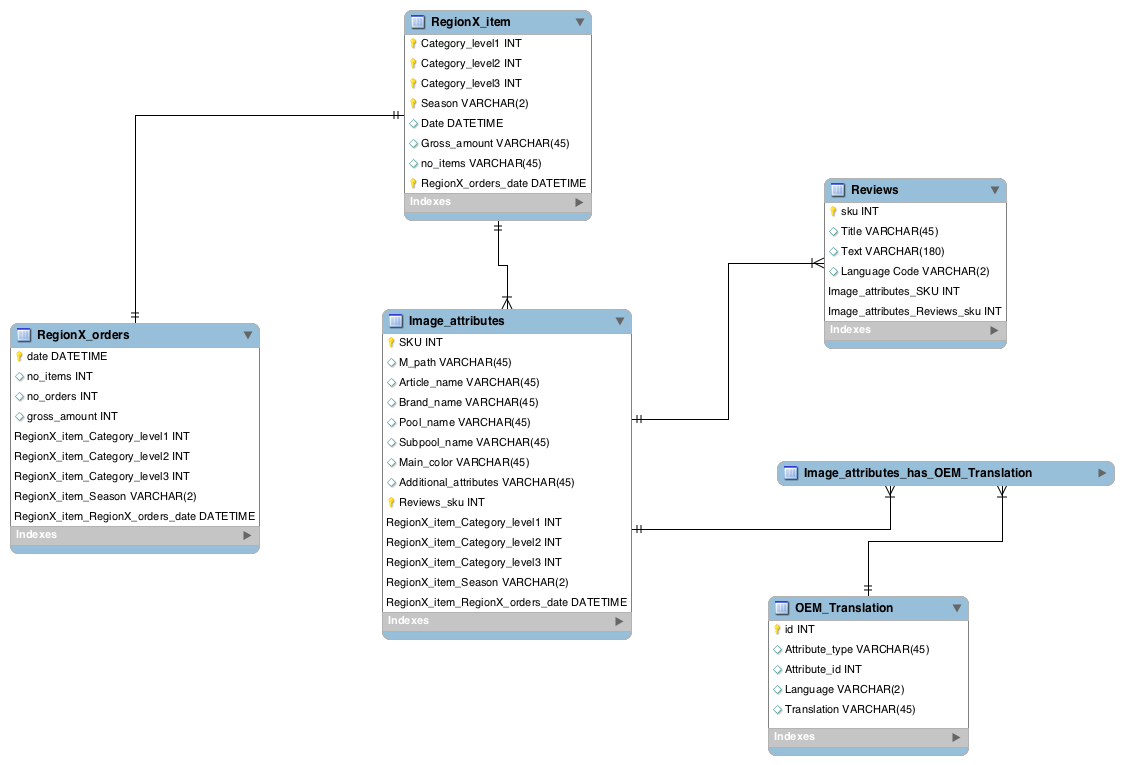
\includegraphics[scale=0.4]{Zalando_RS}
  \caption{Relational model.}
  \label{fig:model_rs}
\end{figure}

%%%%%%%%%%%%%%%%%%%%%%%%%%%%%%%%%%%%%%%%%%%%%%%%%%%%%%%%%%%%%%%%%%%%%%%%%%%%%%%%%%%%%%%%%%%%%%%%%%%%%
%%%%%%%%%%%%%%%%%%%%%%%%%%%%%%%%%%%%%%%%%%%%%%%%%%%%%%%%%%%%%%%%%%%%%%%%%%%%%%%%%%%%%%%%%%%%%%%%%%%%%
\section{Fashion-tech startup}

This section provides an overview of the datasets provided so far by Fashwell. The datasets are in the form of json and csv files. These files are a sample of the data that will be provided by Fashwell. The json files contain brand’s catalogue while the csv files contain a fashion taxonomy. This taxonomy is a fine grained tree of fashion items depending on the gender. We propose to analyse the provided files in order to extract their potential use in terms of research. For the json files, we describe the main attributes and their type. The fashion taxonomy file contains a table of attributes. We describe the most relevant attributes with their respective types. 
We begin by describing two example json files. Each file describes respectively GAP and MACYS online store’s catalogue joined with a schema and an example. These attributes help to extract the product specification, e.g., the categorization of the items will be used in order to build a taxonomy in (WP1).

\paragraph*{dump-example-*.json (* can be GAP or MACYS)}:

\begin{itemize}
    \item Brand (String): Name of Brand
    \item Category (Array of Strings): A categorization hierarchy of the item
    \item Gender (\quotes{enum}: [ \quotes{unisex}, \quotes{female},  \quotes{male}, \quotes{boy}, \quotes{girl}, \quotes{infant}, \quotes{unknown} ]): It could be unisex, female, male, boy, girl, infant or unknown 
    \item Name (String) Name of the item
    \item Internal\_id (String): Internal Order Number
    \item Product\_url (String): Link to the product in the website
    \item Images\_url (Array of Strings): Link to the product image
    \item Desc (String) Gives a description of a product
\end{itemize}

Below we give an example of the json description of one product.

\begin{verbatim}
{ "name": "Nike SB Stefan Janoski Max",
"desc": "The Nike SB Stefan Janoski Max is designed with ...", 
"price": 140.00,			
"msrp": 210.00,
"currency": "EUR",
"sizes": ["34", "38", "40"],
"category": ["men", "accessories", "glasses"],
"images_url": ["http://www.foo.com/bar0.jpg", "http://www.foo.com/bar0.jpg"], 
"gender": "male", "brand": "Nike",
"product_url": "https://www.foo.com/bar/baz",
"ean": 123456789,
"internal_id": "999111",
"features": "110% cotton",
"color": "tomato"
}
\end{verbatim}


Fashwell has different sources of data. In order to have one unique dataset with non redundant elements, they integrate them all together to get one unique fashion tree using the model described in Figure~\ref{fig:classifier}.


\begin{figure}[htb] \centering 
  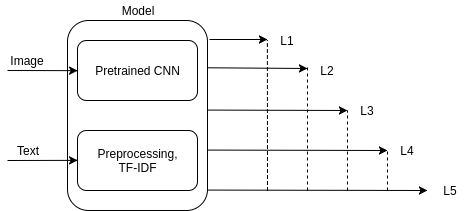
\includegraphics[scale=0.6]{taxonomy_classifier}
  \caption{Fashion items classifier.}
  \label{fig:classifier}
\end{figure}


We provide in what follows a brief description of the model used by Fashwell. This model takes as an input an image and a text associated with one product. For the vision part of the model, a convolutional neural network is used. the model is pre-trained on ImageNet dataset and then fine-tuned to fashion products taxonomy task. The text part of the model uses some NLP techniques for preprocessing, like stemming and stop-word removal, and then uses TF-IDF for feature extraction from the text. In the end, these two parts of the model (vision and text) are combined in a single neural network model which can predict a taxonomy. Interesting finding was that, in most cases, text was much more informative for inferring taxonomy correctly than an image. When a product has multiple images, the classifier is applied on all images with the text describing the product. In a later step, predictions average is made, which usually leads to better results. If there are multiple images per product, the vision part of the model improves in prediction accuracy. This model learns 5 tasks in joint - for each level of taxonomy. The higher the level, the more fine-grained the classification is. It is also taken into consideration the information from the lower levels of predictions to enhance the predictions of higher levels, but still the higher the level, the more imprecise the predictions are. Products with already-labeled taxonomies were used to train the classifier. 

The main attributes of the fashion tree are depicted as follows:

\paragraph*{fashion\_tree\_dump.csv}:

\begin{itemize}
    \item id (Integer): Category id in the Fashwell tree
    \item name (String): Name of the category
    \item parent\_id (Integer): The parents id of a particular category. 
    \item gender (enum: [ \quotes{unisex}, \quotes{female},  \quotes{male}, \quotes{boy}, \quotes{girl},\quotes{infant}, \quotes{unknown} ]): The gender could be any element of the enum set
\end{itemize}

In the following section, we describe the results of the survey on how social media influences the shopping experience of their viewers. This survey aims to help us discovering the platforms and the fashion blogs that are used as fashion drivers. 


\chapter{Fashion Survey}
\label{chap:survey}

Fashion bloggers and social media in a more general way are becoming an influential force within the fashion industry. Fashion related applications pulls data from Instagram and other social media platform in order to enlarge their datasets and consolidate it. The purpose of this survey is to extract more features and discover platforms that are used to spot new clothing trend. In a first part, we present the survey and in the second part, we describe the survey’s analysis and results.

%%%%%%%%%%%%%%%%%%%%%%%%%%%%%%%%%%%%%%%%%%%%%%%%%%%%%%%%%%%%%%%%%%%%%%%%%%%%%%%%%%%%%%%%%%%%%%%%%%
%%%%%%%%%%%%%%%%%%%%%%%%%%%%%%%%%%%%%%%%%%%%%%%%%%%%%%%%%%%%%%%%%%%%%%%%%%%%%%%%%%%%%%%%%%%%%%%%%%
\section{Presentation}
This survey was performed on \ac{CF} asking 800 men and women from 16 European countries questions about their online shopping habits. The choice of the 16 European countries was based on Zalando’s delivery destinations. When the participants accepts the task (or accesses the system web page), they will be asked to read the Information Sheet and Consent Form and indicate their agreement and this is the first page of the system. Then, the participants are given an entry questionnaire to gather demographic information such as age, gender, nationality, etc. Next, each participant will be presented with a series of questions about his/her social media habits, his/her behaviour towards fashion blogs and preferred content presentation in both retailer websites and social media platforms. The results of the survey are described in the following section.

%%%%%%%%%%%%%%%%%%%%%%%%%%%%%%%%%%%%%%%%%%%%%%%%%%%%%%%%%%%%%%%%%%%%%%%%%%%%%%%%%%%%%%%%%%%%%%%%%%
%%%%%%%%%%%%%%%%%%%%%%%%%%%%%%%%%%%%%%%%%%%%%%%%%%%%%%%%%%%%%%%%%%%%%%%%%%%%%%%%%%%%%%%%%%%%%%%%%%
\section{Results and Analysis}
\subsection{Shopping Online/ Social Media Habits}

Online shopping is becoming increasingly popular for multiple reasons. People find it more convenient because it saves time, it is available 24/7 and the comparison between products can be made in few clicks.  Clothes shopping is not an exception, among the 800 men and women we asked, 94.7\% of them shopped clothes online at least once. These digital buyers turn to social media for a variety of reasons like reading comments and discovering new trends. For instance, 75\% of the participants who check their social media account several times a day, use them to follow fashion trend.
While a clear majority use social media to follow new clothing trends, the platform choice differs slightly depending on the age and the gender. Figure~\ref{fig:gender_pref} shows the top platforms depending on the gender. We can see that \ac{FB} is the most popular platform for both men and women, Instagram and \ac{YT} are ranked just behind, then Pinterest who is more popular among women more than men. 

\begin{figure}[htb] \centering 
  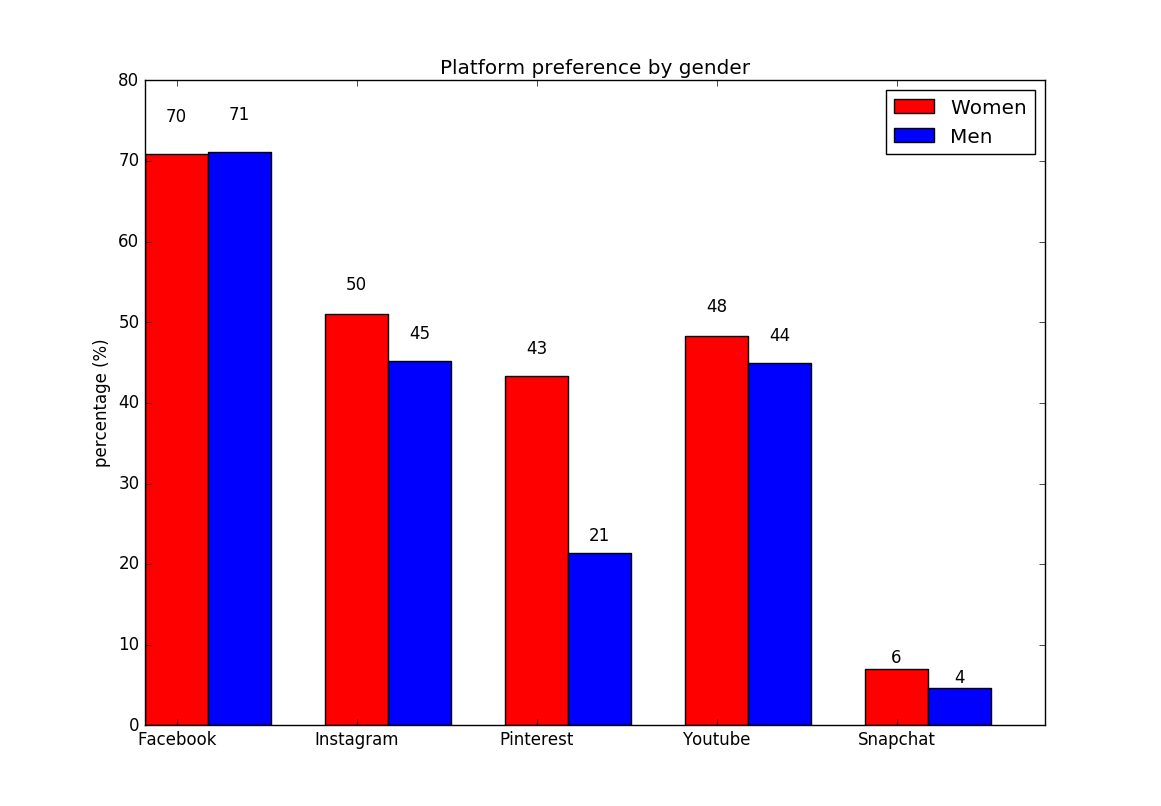
\includegraphics[scale=0.4]{gender_pref}
  \caption{Platform preference by gender.}
  \label{fig:gender_pref}
\end{figure}


The preference for the social media platform depending on the age range is shown in Figure~\ref{fig:age_pref}. \ac{FB} has a uniform and large user base (2 billion monthly active users in 2017) which explains why 70\% of each age range chooses \ac{FB} to discover Fashion trend. Instagram is the second choice with more popularity among the younger generation (under 30). Around half of each age range uses \ac{YT}, then we have Pinterest and Snapchat ranked just behind.


\begin{figure}[htb] \centering 
  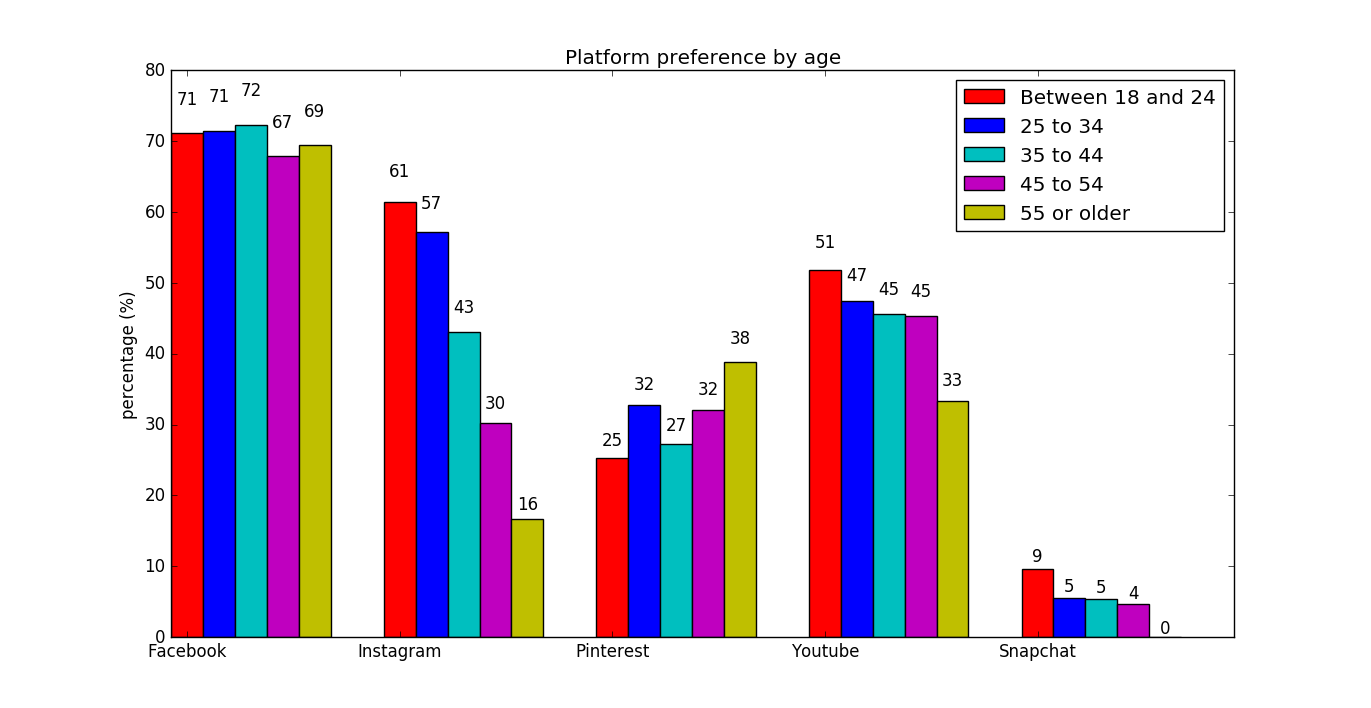
\includegraphics[scale=0.4]{age_pref}
  \caption{ Platform preference for discovering clothing trend by age.}
  \label{fig:age_pref}
\end{figure}



The results of the survey show that the majority of the participants, i.e., 71.8\% of them, uses \ac{FB} platform to discover new fashion trends. When studying the demographic of this majority, around 70\% of each age range uses this platform to discover new trends. This result was expected since the user base of \ac{FB} is uniform. Besides reaching a large community, a \ac{FB} post has more opportunity for getting feedback of all kinds and is more likely to get a deeper level of interaction since the comments can contain text, emoji and images unlike other platforms where only text/emoji are allowed. 

According to the survey results, Instagram is the second platform to be used in order to spot new clothing trends, i.e. 49.1\% of the participants. A majority of these Instagram users are under 30 as a matter of fact, this platform appeals more to the younger generation at the opposite of Pinterest that is slightly more popular in older generations. Almost half of the participants use \ac{YT} to discover fashion. As a matter of fact, in June 2016, beauty-related content generated more than 5 billion views per month. Popular types of \ac{YT} beauty content include tutorials, reviews, and videos produced by beauty vloggers~\cite{stat}.

Since \ac{FB} and Instagram are the most popular platforms to discover fashion according to the survey results, we will briefly describe the difference between the two platforms. \ac{FB} is focused more on text and is largely informational while, Instagram is more about “capturing the moment”. It is also worth mentioning that \ac{FB} content is so diverse that one can easily get distracted, while Instagram focuses on image/video sharing only. Users are more able to be engaged with the visual content shared on Instagram which explains why when asking participants to name fashion influencers they know, we count only 9 \ac{FB} pages while  87 fashion instagram accounts. The difference between the number of \ac{FB} pages and the number of instagram accounts mentioned bring us to conclude that while \ac{FB} has the largest user base, Instagram audience is more engaged. This last result suggests that social media platforms have a key role in creating, advertising and spreading clothing trends. Hence, social media data will play a pivotal role in the rest of our project. Since social media data often comes in an unstructured format, the ensuing data integration task will consist of recognizing key entities to be linked with our fashion catalog (Fashion Knowledge Base), this will be done either via text or image processing.

This question revealed some other platforms used to discover fashion trend like Reddit 21 buttons, google+, Soup.io, lookbook, bantoa, elcorteingles, etc.

\subsection{Influence of Bloggers and Social Media on Their Viewers}

In this section, we gather the results related to how participants use social media to discover fashion trends and who are the influencers they follow to spot new trends.
A common way to stay updated with the latest trend is to follow brands on social media. For instance, 63.6\% of the participants follow their favourite brands on social media. They also find the best way to get inspiration about what clothing to purchase is going through online clothing shops (75.5\%) and by following them on social media (48.6\%). These methods beat by far the traditional way of looking into magazines (27.5\%) and visual merchandising in shops (34.2\%). Therefore, social media platforms are not only used to discover trend but also have an influence on people's decision to purchase items. As shown in the chart of Figure~\ref{fig:freq}, 44.8\% of the participants frequently purchase items discovered through social media. 


\begin{figure}[htb] \centering 
  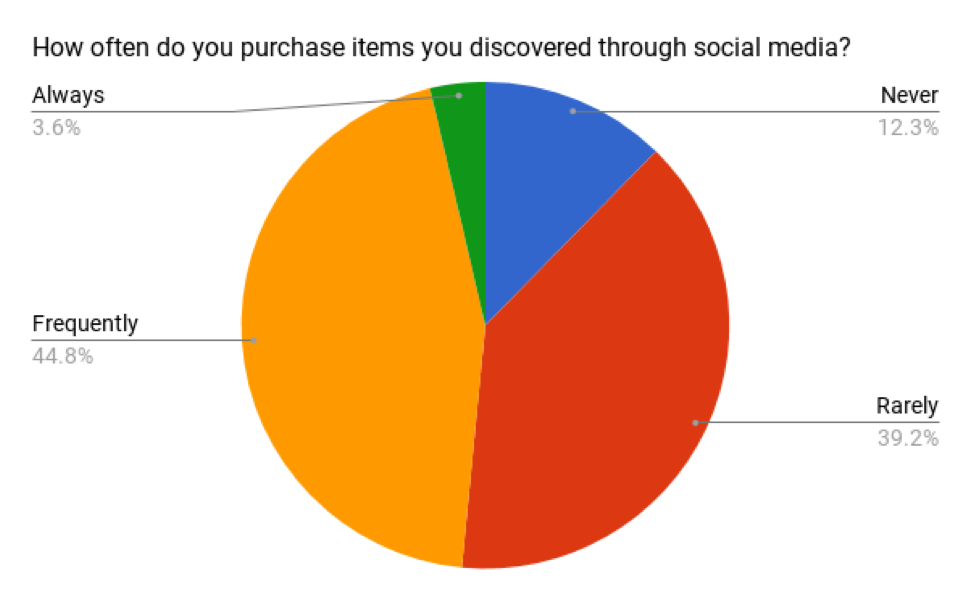
\includegraphics[scale=0.5]{influence_bloggers}
  \caption{Frequency of purchased items discovered through Social Media.}
  \label{fig:freq}
\end{figure}

Below some answers to the question “Describe how you use social media to discover fashion trends”:
“I visit profiles of people who publish photos and reviews of clothes from new collections of well-known brands. I also visit the profiles with ideas how to join various pieces of clothing to make a great and fashionable outlook.”
“\ac{FB} and Twitter are great for discovering new trends, and Pinterest is wonderful for a visual experience.”
These answers reveal how fashion bloggers are gaining a lot of popularity and have a clear influence on their followers as a matter of fact 40\% of the participants use fashion blogs to have an idea about their next shopping.
The participants provided us with 168 distinct blogs, \ac{YT} channels and Instagram accounts (The list is kept in our shared repository). We name here those with the highest number of followers:

\begin{itemize}
    \item @chiaraferragni
    \item @songofstyle 
    \item @galagonzalez
    \item @thefashionguitar
\end{itemize}

From this list we can hypothesis that the list of influencers is large and growing which makes it difficult to keep up manually. The recommendation that we issue for (WP3) is the development of an interface for the continuous collection and curation of an influencer list by means of crowdsourcing.


\subsection{Comments/Reviews}


Users share their feelings and opinions on products mostly to clarify some doubts before purchasing (48.8\%) or to give some subjective feedback afterwards (41\%) as depicted in Figure~\ref{fig:perc}. The most important aspects participants look for in a review are: (i) the item’s general features specially the quality of the product and (ii) whether is it similar to the picture and description.


\begin{figure}[htb] \centering 
  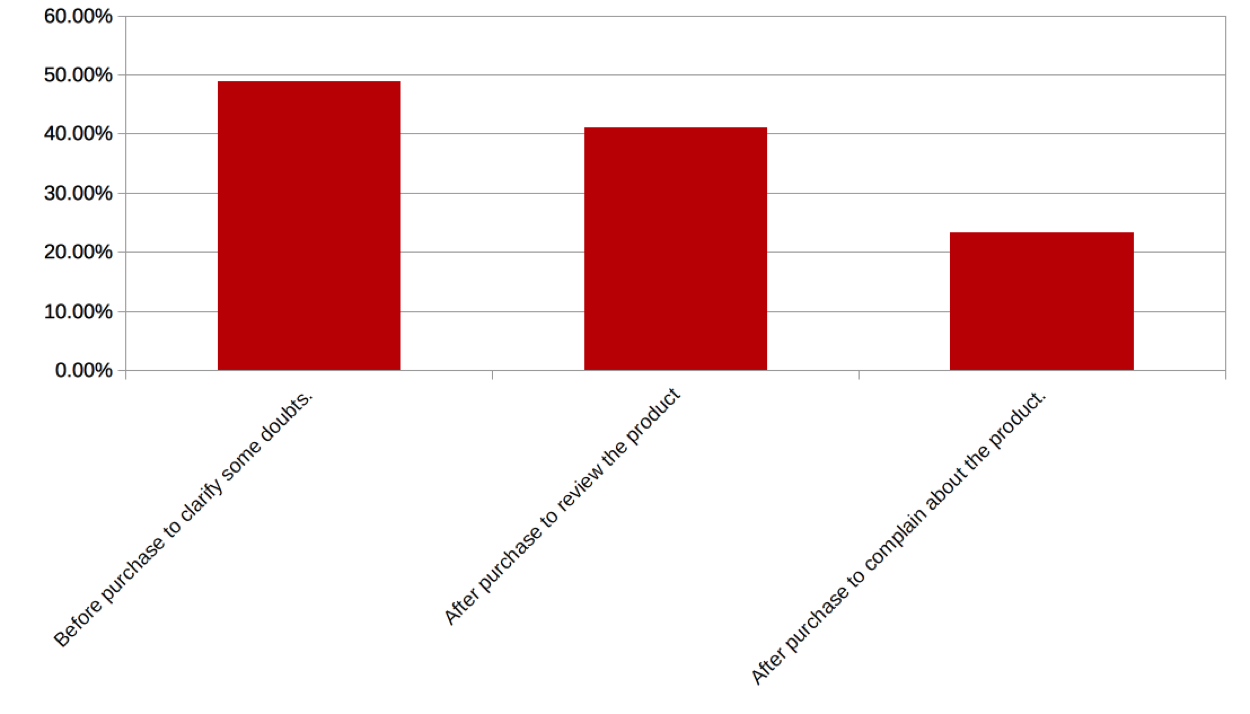
\includegraphics[scale=0.6]{images/figs/comments_reviews}
  \caption{Percentage of participants answering: When are you more likely to review or comment about a fashion product?}
  \label{fig:perc}
\end{figure}


With social media, regular consumers have a direct access to fashion designers, clothing and shoes firms. When fashion companies do social media marketing, they are more able to reach and engage a wider audience. When asking the participants “how do you interact with fashion brands on social media?”, we found as depicted in Figure~\ref{fig:inter} , 43\% of them answering by “liking posts/publications” and 25\% of them by “commenting on posts/publications”. Therefore, it is possible to measure the popularity of a specific trend or style with the number of likes and comments. This same approach was used in different domain such as prediction of the new popular models~\cite{Park:2016:SAI:2818048.2820065} and the box-office performance of newly-released blockbuster movies~\cite{Asur11}.


\begin{figure}[htb] \centering 
  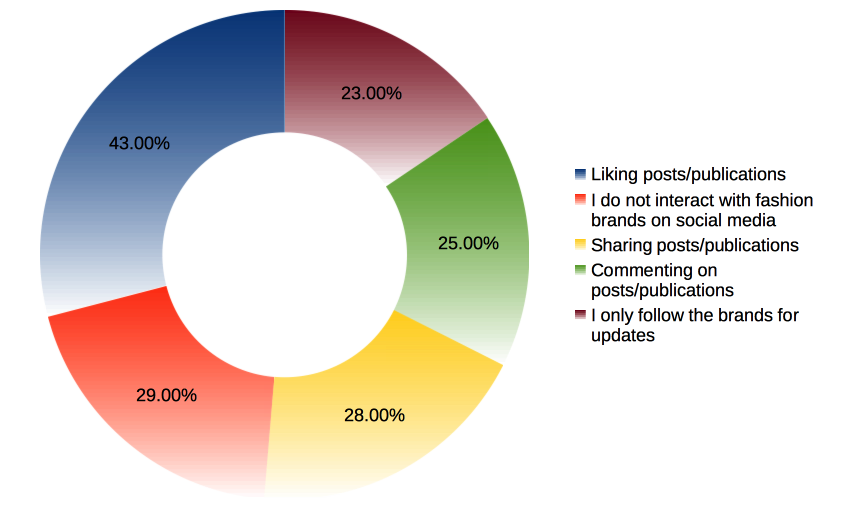
\includegraphics[scale=0.6]{interaction}
  \caption{Interaction with fashion brands.}
  \label{fig:inter}
\end{figure}

\subsection{Fashion Content}

In this section, we describe the preference of data type according to the survey participants  (image, text, videos) and how they prefer items to be displayed.
  
Figure~\ref{fig:content} shows that image is the preferred content users want to see on fashion social media then comes videos and text consecutively. Even though videos seem to have less importance compared to image, they are an important source of information to spot new trends. For example, the participants provided us with around 30 distinct \ac{YT} channels dedicated to fashion. Such a high number of fashion videos shows that the latter are fashion drivers.


\begin{figure}[htb] \centering 
  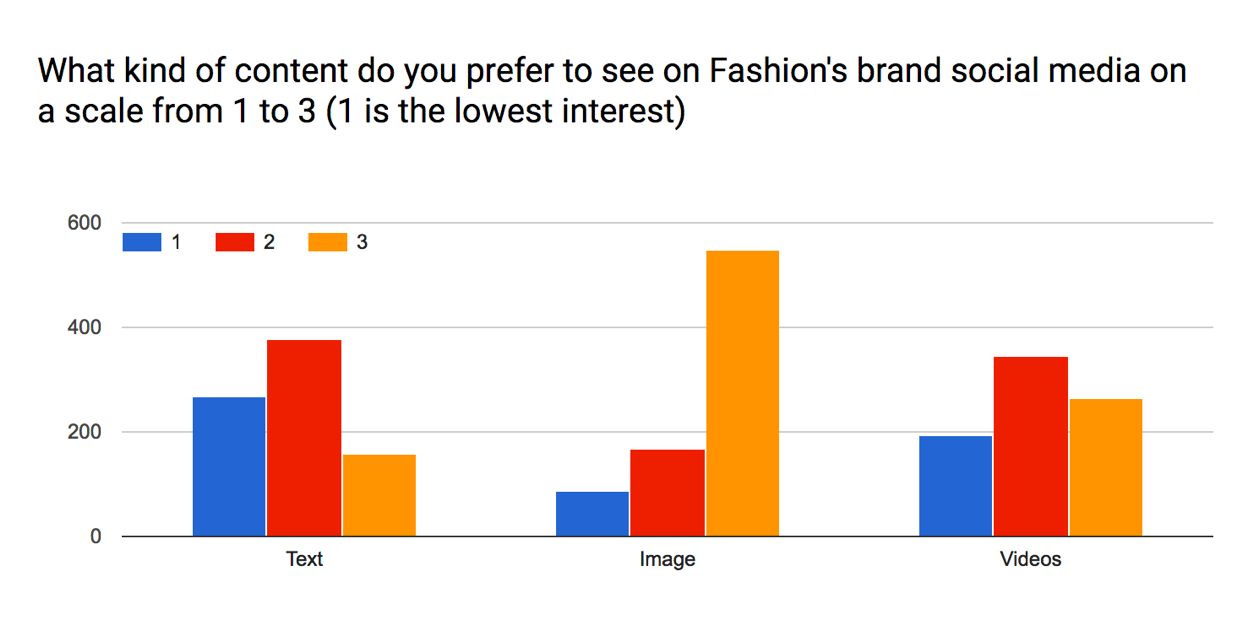
\includegraphics[scale=0.6]{content_pref}
  \caption{Content type preference.}
  \label{fig:content}
\end{figure}



Items on models and showing a combination of items is preferred over focusing on showing items solely as shown in Figure~\ref{fig:focus}. Thus, for the image processing tasks, we recommend to take into account overall style recommendation, i.e., combination of multiple items instead of focusing on showing different items separately.


\begin{figure}[htb] \centering 
  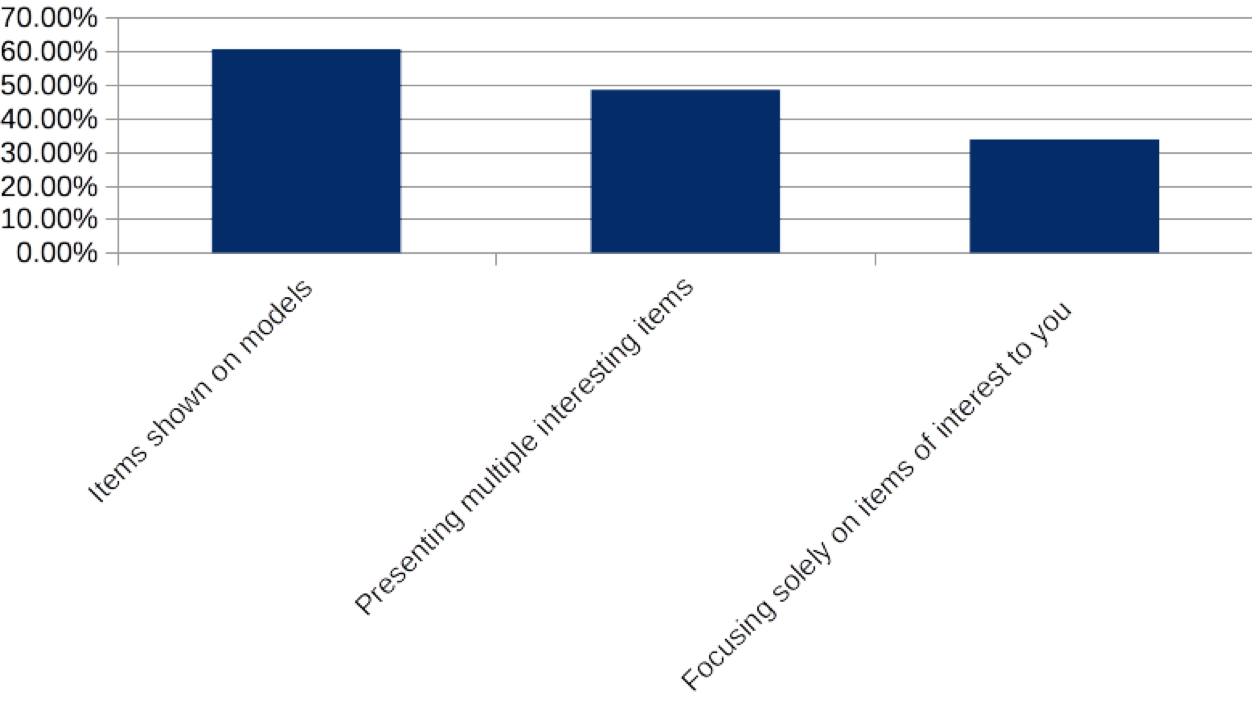
\includegraphics[scale=0.6]{focus_pref}
  \caption{Focus preference.}
  \label{fig:focus}
\end{figure}

\subsection{Other Forms of Content}


VR and AR are still in early development stages. However as technology becomes mainstream, with companies like \ac{FB} and Snapchat investing millions in R\&D, these technologies are expected to be integrated in the social media experience quite soon. Fashion related applications are already launched and even though they were not mentioned by the 800 participants, they will soon become a powerful channel for brand-consumer interaction : 

\begin{itemize}
    \item Uniqlo’s Magic Mirror: Uniqlo offered shoppers the unique ability to imagine themselves in a range of color choices of a single silhouette without the hassle of having to remove the garment.
    \item The Sampler mobile app from Converse: A mobile application that gives people the ability to imagine what a Converse product would look like on-foot without having to actually try on a pair. One has only to point his iPhone camera at his leg and subsequently getting a visual reference on how it would look.
\end{itemize}

We add as a target in WP3 the tracking of the adoption of new technologies.
\chapter{Conclusions}
\label{sec:conc}
In this deliverable, we have described and analyzed all the internal datasets provided by
the FashionBrain partners. This dataset description will help to identify the datasets needed for each task in the project as well as the connections between the provided datasets.  In addition to the dataset description, we have also performed a survey on \ac{CF} to evaluate the importance of \ac{SM} platforms in online shopping. One of the main results of this survey shows that more than 44\% of the social network users frequently purchase items discovered through \ac{SM}, which confirms the increasing importance of \ac{SM} in the fashion industry. The results of this survey will help us identifying
the social platform to focus on for the task of identifying fashion trends using social media (related to D5.5). 


\bibliographystyle{plainnat}
%NOTE - do not duplicate entries in different bib files
\bibliography{bib/references,bib/global}
%\appendix
%\chapter{Appendix}

Example of appendix here
\end{document}
